\section{Kevin Natanel Nainggolan(1174059)}
\subsection{Data Geospasial}
Apa itu DATA GEOSPASIAL, dua kata yang berasal dari geo dan spasial, diamana arti daripada geo sendiri adalah bumi dan spasial berarti raung. Data Geospasial dipecah menjadi dua jenis data, yaitu : 
\begin {enumerate}
	\item Data Grafis, terdiri dari tiga elemen, diantaranya:
		\begin {itemize}
			\item Titik
			\item Garis
			\item Luasan
		\end {itemize}
	\item Data Atribut
\end {enumerate}

\subsubsection{Tipe Data Vektor}
Data Vektor digunakan pada Geospasil pada titik koordinat yang menampilkan, menempatkan, dan menyimpan data spacial dengan elemen data grafis atau geometri, seperti yang sudah dibahas diatas, terdapat beberapa jenis tipe data vektor, diantaranya: 
\begin {itemize}
	\item Titik
	\item Garis
	\item Polygon
\end {itemize}
Tipe data yang sudah dituliskan di atas biasanya terletak pada peta, dan setiap bagian dari data tersebut bisa mempunyai informasi yang berhubungan satu dengan yang lainnya

\subsubsection{Tipe Data Line}
Data Line atau garis berbentuk satu dimensi yang menghubungkan dua titik atau lebih, biasanya Data Line digunakan untuk menunjukan objek geometri linear. Hal ini yang akan bergantung pada peta karena menjadi sumber atau skala representasi sebagai objek dengan menampilkan bentuk geometri garis.

\subsubsection{Raster}
Data grid atau raster mewakili tipe fitur permukaan, data ini berbasis sel dengan kategori data yang mencangkup citra udara dan satelit. Berikut jenis data raster:
\begin {itemize}
	\item Kontinu
	\item Diskrit
\end {itemize}

 
\subsection{Link}
\href {} Klik disini Untuk video dari geospasial selengkapnya
\subsection{Plagiarism}
\begin{figure}[H]
	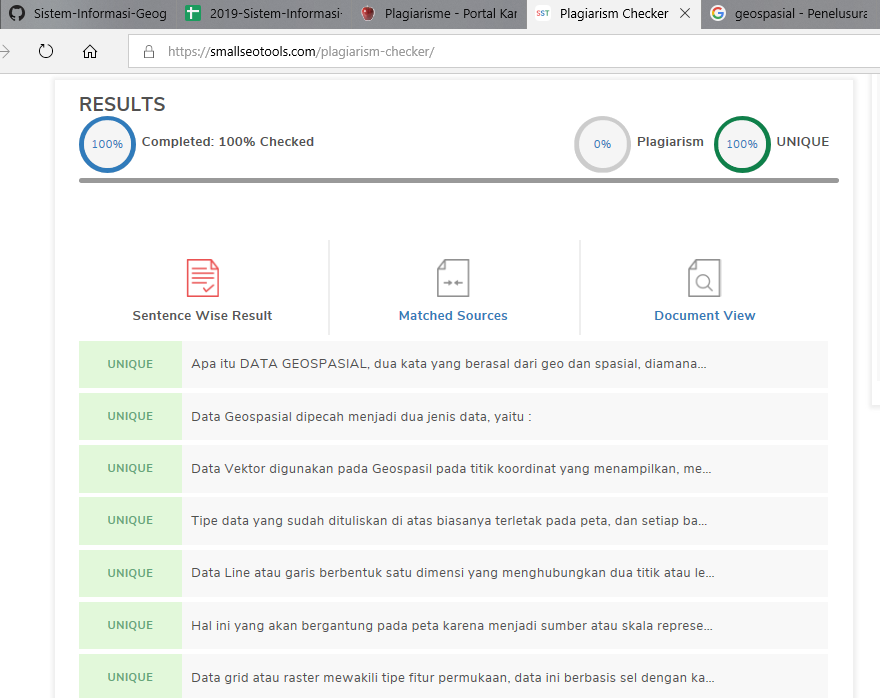
\includegraphics[width=4cm]{figures/1174059/plagiarisme.png}
	\centering
	\caption{Check Plagiat Kevin}
\end{figure}

